\section{Methodology}
\label{sec:method}

\subsection{Construction Embodied World Graph}

The intermediate representation is implemented as a Construction Embodied
World Graph (CEWG). Its typed nodes contain components, assembly interfaces,
construction states, robots, tools, tasks, work zones, robot capabilities, and
provenance records. Edges make cross-entity claims explicit, including
\texttt{located\_in}, \texttt{has\_interface}, \texttt{mates\_with},
\texttt{performed\_by}, \texttt{uses\_tool}, \texttt{targets}, and
\texttt{can\_transition\_to}. It is deliberately simulator-neutral so that IFC
extraction, graph-integrity checks, USD authoring, scene validation, and
runtime adapters remain separately testable.

\Cref{fig:architecture} shows how these modules form one auditable compilation
pipeline. Data artefacts are identified on the arrows so that implementation
outputs, validation evidence, and runtime measurements can be traced back to
their source.

\begin{figure*}[t]
\centering
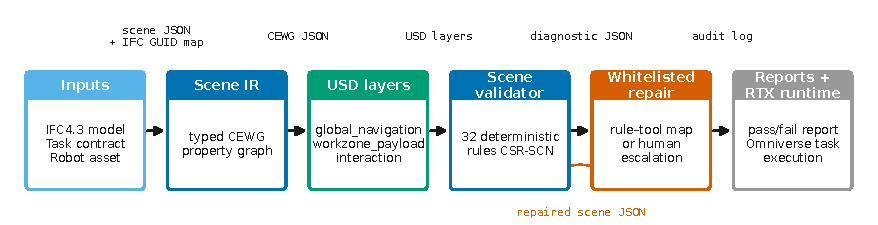
\includegraphics[width=\textwidth]{figures/fig02_architecture.pdf}
\caption{Architecture of \systemname. Deterministic compilation and validation
remain separate from agentic diagnosis and from the downstream simulation
runtime.}
\label{fig:architecture}
\end{figure*}

The typed entities and relations are specified in
\Cref{fig:intermediate-representation}. The figure also exposes provenance as
part of the representation rather than as an external note attached after
simulation.

\begin{figure*}[t]
\centering
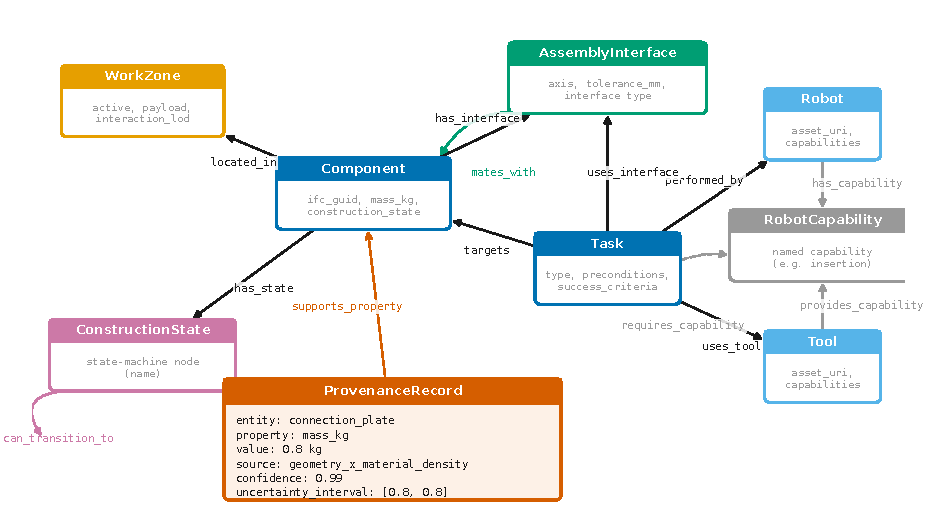
\includegraphics[width=\textwidth]{figures/fig03_intermediate_representation.pdf}
\caption{Construction Embodied World Graph and
property-level provenance. The same engineering identity connects source IFC
entities, composed USD prims, task targets, and validation evidence.}
\label{fig:intermediate-representation}
\end{figure*}

\subsection{Task-activated multi-scale compilation}

The compiler maps building circulation and architectural boundaries to a
coarse global layer. It emits each work zone as an independently loadable
payload and reserves interface-level geometry, tolerances, contact properties,
and temporary constraints for the active interaction layer. IFC GUIDs remain
stable across all layers.

\Cref{fig:multiscale-composition} illustrates the OpenUSD composition. Its
purpose is \emph{working-set management}, not runtime acceleration: only the
global layer and the active interaction layer are composed, so the loaded
prim set tracks the active task rather than the whole model
(\Cref{sec:results} reports the measured working-set reduction; load time and
peak memory are small and comparable across modes, so we do not claim a
runtime-performance advantage).

\begin{figure*}[t]
\centering
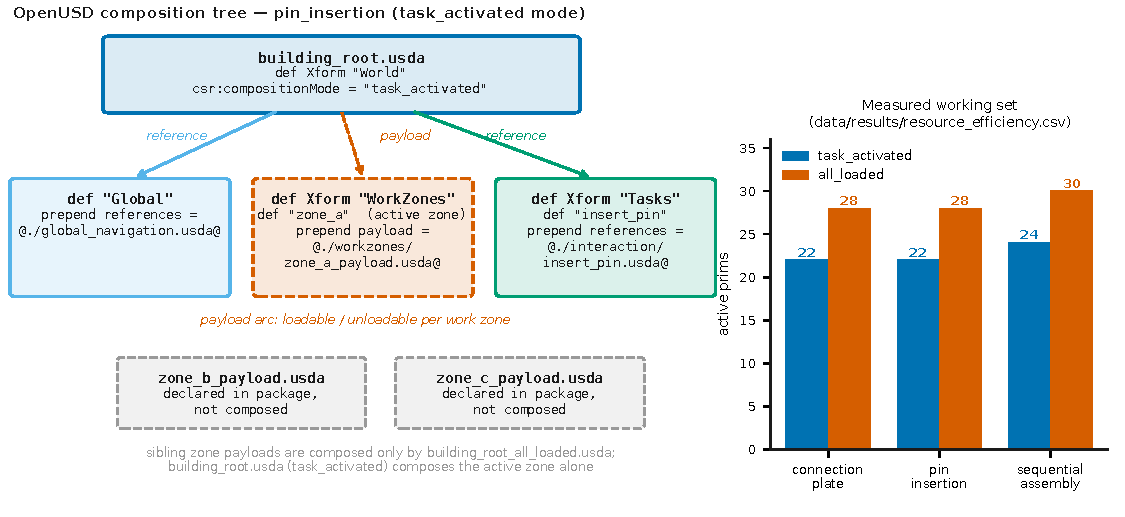
\includegraphics[width=\textwidth]{figures/fig04_multiscale_composition.pdf}
\caption{Task-activated multi-scale scene composition. Fine contact geometry
and temporary constraints are loaded only for the active interaction while
engineering identity is preserved across layers.}
\label{fig:multiscale-composition}
\end{figure*}

\subsection{Construction scene readiness contract}

Rules are grouped into identity and reference closure, coordinate and unit
consistency, interface and tolerance completeness, state-transition validity,
robot capability and task preconditions, physical stability, provenance, and
multi-scale fidelity. Each rule is deterministic and emits a machine-readable
failure.

\Cref{tab:contract} freezes the contract categories and the evidence required
from the implementation. The full list of versioned rules and unit tests will
be released as supplementary material rather than compressed into the main
text.

\begin{table*}[t]
\centering
\caption{Construction-scene readiness contract (v0.3.0, 30 rules). Rule
identifiers and per-scenario coverage are reported in the supplementary
material.}
\label{tab:contract}
\small
\resizebox{\textwidth}{!}{%
\begin{tabular}{p{0.16\textwidth}p{0.23\textwidth}p{0.19\textwidth}
p{0.10\textwidth}p{0.22\textwidth}}
\toprule
Contract category & Required scene evidence & Deterministic check &
Severity & Consequence if violated \\
\midrule
Identity and closure & IFC GUID, USD prim path, closed task and asset
references & Uniqueness and reference resolution & Critical & Wrong or
unresolved task object \\
Spatial consistency & Units, up axis, frames, transform chain, work-zone
membership & Transform normalization and bounds & Critical & Unreachable or
misplaced interaction \\
Assembly interface & Paired interface, insertion axis, tolerance, grasp and
support regions & Geometric and relational constraints & Critical & False
alignment or infeasible insertion \\
Construction state & Current state, legal predecessor, action precondition,
completion criterion & State-machine validation & Critical & Unsafe or
meaningless action \\
Physics and stability & Mass, inertia, collision, contact property, temporary
support & Physical admissibility and support tests & Critical or major & Unstable
or non-physical simulation \\
Provenance and fidelity & Property source, confidence, uncertainty, activated
payload and level of detail & Authority and task-fidelity policy & Major &
Unauditable result or hidden interaction error \\
\bottomrule
\end{tabular}
}
\end{table*}

\subsection{Validator-grounded repair}

The repair agent receives no free-form authority over the scene. It may inspect
evidence, select a permitted tool, propose bounded parameters, execute the tool,
and request re-validation. Unsupported or high-risk changes are escalated.

\begin{figure*}[t]
\centering
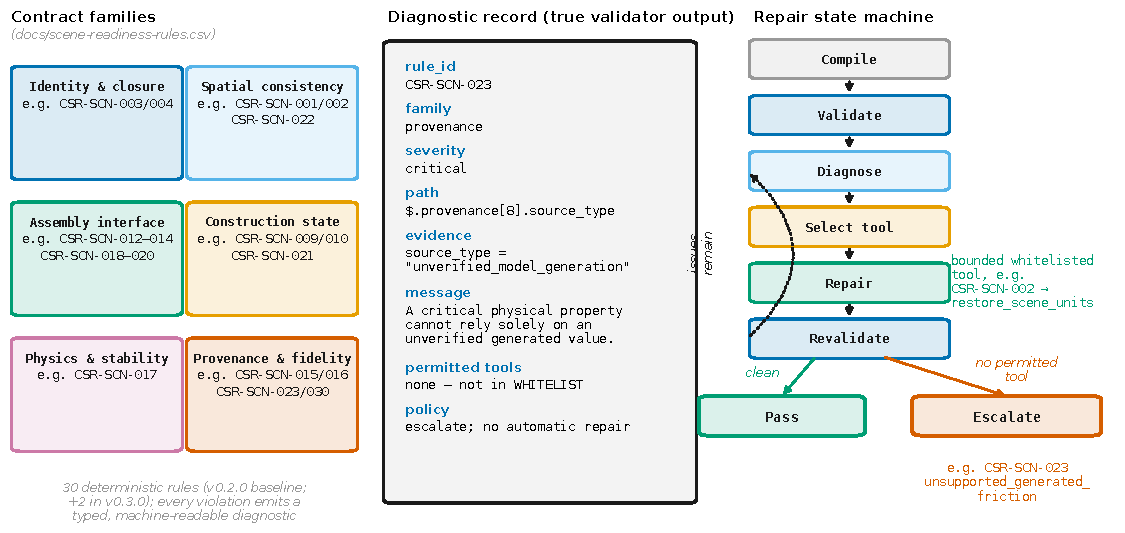
\includegraphics[width=\textwidth]{figures/fig05_repair_loop.pdf}
\caption{Validator-grounded repair. The agent interprets structured evidence
and selects a bounded operation, whereas deterministic rules decide acceptance
and high-risk or unsupported mutations are escalated.}
\label{fig:repair-loop}
\end{figure*}
